Range scans with panoramic angular ranges induce fewer pose ambiguities in
rank-fields than those with non-panoramic field of view. In the latter case
this means that, given the evidence of subsections \ref{subsec:exp_a} and
\ref{subsec:exp_c} where $\lambda = 3\pi/2$ rad, the choice of $k=10$ largely
inhibits the propagation of ambiguities to the output (fig.
\ref{fig:c:errors_and_time}).  However, non-panoramic sensors coupled
with repeated environment structures may give rise to the conditions of figure
\ref{fig:h_and_h_not_fig} (bottom). Other sources of potential, large pose
errors for CBGL are portrayed in figure \ref{fig:a:map_and_trajectory}: (a)
regions coloured with cyan indicate closed glass doors, wherein high range
errors result in discrepancy with map-derived virtual ranges, which is
subsequently propagated to $\psi$-fields and hence $\texttt{r}$-fields, and (b)
regions coloured purple indicate vicinities around doors, wherein
higher locational density or values of $k$ may be required to suppress pose
ambiguities propagated to $\texttt{r}$-fields.

\begin{figure}
  \definecolor{v}{RGB}{131, 186, 109}
\definecolor{x}{RGB}{217, 33, 32}
\definecolor{w}{RGB}{120, 28, 130}

% GNUPLOT: LaTeX picture with Postscript
\begingroup
  \makeatletter
  \providecommand\color[2][]{%
    \GenericError{(gnuplot) \space\space\space\@spaces}{%
      Package color not loaded in conjunction with
      terminal option `colourtext'%
    }{See the gnuplot documentation for explanation.%
    }{Either use 'blacktext' in gnuplot or load the package
      color.sty in LaTeX.}%
    \renewcommand\color[2][]{}%
  }%
  \providecommand\includegraphics[2][]{%
    \GenericError{(gnuplot) \space\space\space\@spaces}{%
      Package graphicx or graphics not loaded%
    }{See the gnuplot documentation for explanation.%
    }{The gnuplot epslatex terminal needs graphicx.sty or graphics.sty.}%
    \renewcommand\includegraphics[2][]{}%
  }%
  \providecommand\rotatebox[2]{#2}%
  \@ifundefined{ifGPcolor}{%
    \newif\ifGPcolor
    \GPcolorfalse
  }{}%
  \@ifundefined{ifGPblacktext}{%
    \newif\ifGPblacktext
    \GPblacktexttrue
  }{}%
  % define a \g@addto@macro without @ in the name:
  \let\gplgaddtomacro\g@addto@macro
  % define empty templates for all commands taking text:
  \gdef\gplfronttext{}%
  \gdef\gplfronttext{}%
  \makeatother
  \ifGPblacktext
    % no textcolor at all
    \def\colorrgb#1{}%
    \def\colorgray#1{}%
  \else
    % gray or color?
    \ifGPcolor
      \def\colorrgb#1{\color[rgb]{#1}}%
      \def\colorgray#1{\color[gray]{#1}}%
      \expandafter\def\csname LTw\endcsname{\color{white}}%
      \expandafter\def\csname LTb\endcsname{\color{black}}%
      \expandafter\def\csname LTa\endcsname{\color{black}}%
      \expandafter\def\csname LT0\endcsname{\color[rgb]{1,0,0}}%
      \expandafter\def\csname LT1\endcsname{\color[rgb]{0,1,0}}%
      \expandafter\def\csname LT2\endcsname{\color[rgb]{0,0,1}}%
      \expandafter\def\csname LT3\endcsname{\color[rgb]{1,0,1}}%
      \expandafter\def\csname LT4\endcsname{\color[rgb]{0,1,1}}%
      \expandafter\def\csname LT5\endcsname{\color[rgb]{1,1,0}}%
      \expandafter\def\csname LT6\endcsname{\color[rgb]{0,0,0}}%
      \expandafter\def\csname LT7\endcsname{\color[rgb]{1,0.3,0}}%
      \expandafter\def\csname LT8\endcsname{\color[rgb]{0.5,0.5,0.5}}%
    \else
      % gray
      \def\colorrgb#1{\color{black}}%
      \def\colorgray#1{\color[gray]{#1}}%
      \expandafter\def\csname LTw\endcsname{\color{white}}%
      \expandafter\def\csname LTb\endcsname{\color{black}}%
      \expandafter\def\csname LTa\endcsname{\color{black}}%
      \expandafter\def\csname LT0\endcsname{\color{black}}%
      \expandafter\def\csname LT1\endcsname{\color{black}}%
      \expandafter\def\csname LT2\endcsname{\color{black}}%
      \expandafter\def\csname LT3\endcsname{\color{black}}%
      \expandafter\def\csname LT4\endcsname{\color{black}}%
      \expandafter\def\csname LT5\endcsname{\color{black}}%
      \expandafter\def\csname LT6\endcsname{\color{black}}%
      \expandafter\def\csname LT7\endcsname{\color{black}}%
      \expandafter\def\csname LT8\endcsname{\color{black}}%
    \fi
  \fi
    \setlength{\unitlength}{0.0500bp}%
    \ifx\gptboxheight\undefined%
      \newlength{\gptboxheight}%
      \newlength{\gptboxwidth}%
      \newsavebox{\gptboxtext}%
    \fi%
    \setlength{\fboxrule}{0.5pt}%
    \setlength{\fboxsep}{1pt}%

\hspace{0.25cm}
\begin{picture}(4600.00,3500.00)%
    \gplgaddtomacro\gplfronttext{%
      \colorrgb{0.15,0.15,0.15}%
      \put(428,1925){\makebox(0,0)[r]{\strut{}\footnotesize $0$}}%
      \colorrgb{0.15,0.15,0.15}%
      \put(428,2129){\makebox(0,0)[r]{\strut{}\footnotesize $\psi_0$}}%
      \colorrgb{0.15,0.15,0.15}%
      \put(428,2333){\makebox(0,0)[r]{\strut{}\footnotesize $400$}}%
      \colorrgb{0.15,0.15,0.15}%
      \put(428,2741){\makebox(0,0)[r]{\strut{}\footnotesize $800$}}%
      \colorrgb{0.15,0.15,0.15}%
      \put(428,3149){\makebox(0,0)[r]{\strut{}\footnotesize $1200$}}%
      \colorrgb{0.15,0.15,0.15}%
      \put(460,1755){\makebox(0,0){\strut{}\footnotesize $0.05$}}%
      \colorrgb{0.15,0.15,0.15}%
      \put(1378,1755){\makebox(0,0){\strut{}\footnotesize $\delta_0$}}%
      \colorrgb{0.15,0.15,0.15}%
      \put(1659,1755){\makebox(0,0){\strut{}\footnotesize $1.5$}}%
      \colorrgb{0.15,0.15,0.15}%
      %\put(1903,2705){\makebox(0,0){\strut{}\footnotesize $3.0$}}%
      \colorrgb{0.15,0.15,0.15}%
      \put(2046,1755){\makebox(0,0){\strut{}\footnotesize $4.5$}}%
    }%
    \gplgaddtomacro\gplfronttext{%
      \colorrgb{0.15,0.15,0.15}%
      \put(-150,2537){\rotatebox{90}{\makebox(0,0){\strut{}\footnotesize CAER [m]}}}%
    }%
    \gplgaddtomacro\gplfronttext{%
      \colorrgb{0.15,0.15,0.15}%
      \put(2935,1925){\makebox(0,0)[r]{\strut{}\footnotesize $10^0$}}%
      \colorrgb{0.15,0.15,0.15}%
      \put(2935,2168){\makebox(0,0)[r]{\strut{}\footnotesize $10^1$}}%
      \colorrgb{0.15,0.15,0.15}%
      \put(2935,2411){\makebox(0,0)[r]{\strut{}\footnotesize $10^2$}}%
      \colorrgb{0.15,0.15,0.15}%
      \put(2935,2655){\makebox(0,0)[r]{\strut{}\footnotesize $10^3$}}%
      \colorrgb{0.15,0.15,0.15}%
      \put(2935,2898){\makebox(0,0)[r]{\strut{}\footnotesize $10^4$}}%
      \colorrgb{0.15,0.15,0.15}%
      \put(2935,3141){\makebox(0,0)[r]{\strut{}\footnotesize $10^5$}}%
      \colorrgb{0.15,0.15,0.15}%
      \put(2967,1755){\makebox(0,0){\strut{}\footnotesize $0.05$}}%
      \colorrgb{0.15,0.15,0.15}%
      \put(3885,1755){\makebox(0,0){\strut{}\footnotesize $\delta_0$}}%
      \colorrgb{0.15,0.15,0.15}%
      \put(4166,1755){\makebox(0,0){\strut{}\footnotesize $1.5$}}%
      \colorrgb{0.15,0.15,0.15}%
      %\put(4410,2705){\makebox(0,0){\strut{}\footnotesize $3.0$}}%
      \colorrgb{0.15,0.15,0.15}%
      \put(4553,1755){\makebox(0,0){\strut{}\footnotesize $4.5$}}%
    }%
    \gplgaddtomacro\gplfronttext{%
      \colorrgb{0.15,0.15,0.15}%
      \put(2400,2537){\rotatebox{90}{\makebox(0,0){\strut{}\footnotesize Hypotheses' ranks}}}%
    }%
    \gplgaddtomacro\gplfronttext{%
      \colorrgb{0.15,0.15,0.15}%
      \put(428,441){\makebox(0,0)[r]{\strut{}\footnotesize $\psi_0$}}%
      \colorrgb{0.15,0.15,0.15}%
      \put(428,979){\makebox(0,0)[r]{\strut{}\footnotesize $500$}}%
      \colorrgb{0.15,0.15,0.15}%
      \put(428,1244){\makebox(0,0)[r]{\strut{}\footnotesize $1000$}}%
      \colorrgb{0.15,0.15,0.15}%
      \put(428,1510){\makebox(0,0)[r]{\strut{}\footnotesize $2000$}}%
      \colorrgb{0.15,0.15,0.15}%
      \put(460,180){\makebox(0,0){\strut{}\footnotesize $0.05$}}%
      \colorrgb{0.15,0.15,0.15}%
      \put(854,180){\makebox(0,0){\strut{}\footnotesize $5.0$}}%
      \colorrgb{0.15,0.15,0.15}%
      \put(1251,180){\makebox(0,0){\strut{}\footnotesize $10.0$}}%
      \colorrgb{0.15,0.15,0.15}%
      \put(1635,180){\makebox(0,0){\strut{}\footnotesize $\delta_0$}}%
      \colorrgb{0.15,0.15,0.15}%
      \put(2046,180){\makebox(0,0){\strut{}\footnotesize $20.0$}}%
    }%
    \gplgaddtomacro\gplfronttext{%
      \colorrgb{0.15,0.15,0.15}%
      \put(-150,962){\rotatebox{90}{\makebox(0,0){\strut{}\footnotesize CAER [m]}}}%
    }%
    \gplgaddtomacro\gplfronttext{%
      \colorrgb{0.15,0.15,0.15}%
      \put(2935,350){\makebox(0,0)[r]{\strut{}\footnotesize $10^0$}}%
      \colorrgb{0.15,0.15,0.15}%
      \put(2935,554){\makebox(0,0)[r]{\strut{}\footnotesize $10^1$}}%
      \colorrgb{0.15,0.15,0.15}%
      \put(2935,758){\makebox(0,0)[r]{\strut{}\footnotesize $10^2$}}%
      \colorrgb{0.15,0.15,0.15}%
      \put(2935,962){\makebox(0,0)[r]{\strut{}\footnotesize $10^3$}}%
      \colorrgb{0.15,0.15,0.15}%
      \put(2935,1166){\makebox(0,0)[r]{\strut{}\footnotesize $10^4$}}%
      \colorrgb{0.15,0.15,0.15}%
      \put(2935,1369){\makebox(0,0)[r]{\strut{}\footnotesize $10^5$}}%
      \colorrgb{0.15,0.15,0.15}%
      \put(2935,1573){\makebox(0,0)[r]{\strut{}\footnotesize $10^6$}}%
      \colorrgb{0.15,0.15,0.15}%
      \put(2967,180){\makebox(0,0){\strut{}\footnotesize $0.05$}}%
      \colorrgb{0.15,0.15,0.15}%
      \put(3361,180){\makebox(0,0){\strut{}\footnotesize $5.0$}}%
      \colorrgb{0.15,0.15,0.15}%
      \put(3758,180){\makebox(0,0){\strut{}\footnotesize $10.0$}}%
      \colorrgb{0.15,0.15,0.15}%
      \put(4142,180){\makebox(0,0){\strut{}\footnotesize $\delta_0$}}%
      \colorrgb{0.15,0.15,0.15}%
      \put(4553,180){\makebox(0,0){\strut{}\footnotesize $20.0$}}%
    }%
    \gplgaddtomacro\gplfronttext{%
      \colorrgb{0.15,0.15,0.15}%
      \put(2400,962){\rotatebox{90}{\makebox(0,0){\strut{}\footnotesize Hypotheses' ranks}}}%
      \colorrgb{0.15,0.15,0.15}%
      \put(2300,-100){\makebox(0,0){\strut{}\footnotesize Estimate error $\delta$ \footnotesize [(m$^2$ + rad$^2$)$^{1/2}$]}}%

      \put(1300,3300){\makebox(0,0){\makebox(0,0){\strut{}{\color{v}{\rule[0.6mm]{0.5cm}{0.75mm}}} $\mathcal{V}$}}}%
      \put(2300,3300){\makebox(0,0){\makebox(0,0){\strut{}{\color{x}{\rule[0.6mm]{0.5cm}{0.75mm}}} $\mathcal{X}$}}}%
      \put(3300,3300){\makebox(0,0){\makebox(0,0){\strut{}{\color{w}{\rule[0.6mm]{0.5cm}{0.75mm}}} $\mathcal{W}$}}}%
    }%
    \put(0,0){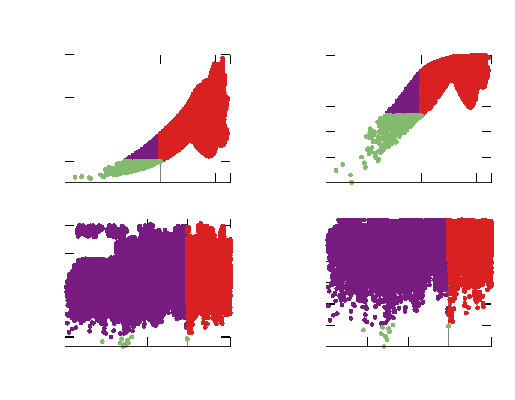
\includegraphics{./figures/h_and_h_not_fig}}%
    \gplfronttext
  \end{picture}%
\endgroup

  \vspace{0.3cm}
  \caption{\small The $\psi$-field (left) and \texttt{r}-field (right) of a
           configuration where Observation \ref{obs:observation_o} may (top)
           and may not (bottom) be made for $\delta \leq \delta_0$. Bottom:
           in contrast to the top row, set $\mathcal{V}$ is empty of admissible
           pose estimates for $\delta < 4.5 \ (\text{m}^2 +
           \text{rad}^2)^{1/2}$. The effect is produced in environment
           WILLOWGARAGE (pose $\bm{p}_{i}^G$; subsection \ref{subsec:exp_b})
           due to (a) the repetition of the immediate environment of the sensor
           more than once in the given map, and (b) the non-panoramic angular
           range of the sensor}
  \vspace{-0.5cm}
  \label{fig:h_and_h_not_fig}
\end{figure}
